\documentclass[11pt,a4paper]{article}

% ---------- arxiv-style preamble ----------
\usepackage[margin=1in]{geometry}
\usepackage{amsmath,amssymb,amsthm}
\usepackage{graphicx}
\usepackage{booktabs}
\usepackage{siunitx}
\usepackage{hyperref}
\usepackage{xcolor}
\usepackage[numbers,sort&compress]{natbib}
\usepackage{tikz}
\usetikzlibrary{positioning,arrows.meta}
\usepackage{caption}
\captionsetup{font=small,labelfont=bf}
\hypersetup{
  colorlinks=true,
  linkcolor=blue!50!black,
  citecolor=blue!50!black,
  urlcolor=blue!50!black
}

% honest-stance shorthands
\definecolor{honestgreen}{HTML}{2E7D32}
\definecolor{honestred}{HTML}{C62828}

\title{
  \textbf{First-Principles Reproduction of H\textsubscript{3}S Critical Temperature via $q$-Grid Convergence}\\[4pt]
  \large Textbook-Accuracy Measurement Match (175--195\,K vs.\ 203\,K) Where Ambient-Trained ML Fails by Two Orders of Magnitude
}

\author{
  Min Woo Park\\
  \normalsize\textit{dancinlab}\\[2pt]
  \normalsize\href{https://github.com/dancinlab}{\texttt{github.com/dancinlab}}
  \thanks{Source repositories:
    \url{https://github.com/dancinlab/demiurge},
    \url{https://github.com/dancinlab/hexa-lang}.}
}

\date{2026-05-22}

\begin{document}

\maketitle

% =========================================================================
\begin{abstract}
We test whether harmonic density-functional theory electron--phonon coupling reproduces
the measured superconducting transition temperature of cubic Im\textendash 3\textendash m
H\textsubscript{3}S \cite{drozdov2015h3s} once the phonon Brillouin-zone sampling is
converged. Two ambient-trained graph neural networks (BETE-NET \cite{gibson2025betenet}
and ALIGNN \cite{choudhary2022alignn}) under-predict the electron-phonon coupling
constant $\lambda$ by a factor of $4$--$5$ on the hydride family; the failure is
localised to $\lambda$ while $\omega_{\log}$ is roughly correct, ruling out structure
quality as the cause. Driving Quantum ESPRESSO 7.5 \cite{giannozzi2009qe,giannozzi2017qe}
electron--phonon DFPT on a converged $24^3$ $k$-grid with $q$-grid densified from
$2{\times}2{\times}2 \to 4{\times}4{\times}4 \to 6{\times}6{\times}6$ raises $\lambda$
monotonically from $0.85 \to 1.3 \to \mathbf{2.1\text{--}2.6}$, matching the harmonic
literature value $\lambda \approx 2.2$ \cite{errea2016h3s}. The Allen--Dynes
\cite{allendynes1975} critical temperature at the $6{\times}6{\times}6$-$q$ grid is
$T_c^{\text{AD}} = 175$--$195$\,K ($\mu^*=0.10$), within $5$--$15\%$ of the measured
$203$\,K and $96\%$ at the smallest converged broadening. We make no claim of
room-temperature superconductivity: H\textsubscript{3}S requires $\sim 150$\,GPa and
remains below the ambient gate. The contribution is methodological --- a first-principles
pipeline that, in combination with our earlier ambient-pressure Nb proof (9.9\,K vs.\
measured 9.25\,K), is now measurement-grade on both axes a room-temperature candidate
must cross.
\end{abstract}

% =========================================================================
\section{Introduction}
\label{sec:intro}

Conventional Bardeen--Cooper--Schrieffer \cite{bcs1957} superconductivity in dense
hydrides has produced a series of measured transition temperatures climbing toward room
temperature: H\textsubscript{3}S at $203$\,K \cite{drozdov2015h3s}, LaH\textsubscript{10}
near $250$\,K, YH\textsubscript{6} at $224$\,K, all in the $150$--$200$\,GPa range. The
underlying mechanism is strong electron--phonon coupling on the high-frequency hydrogen
sublattice, with coupling constant $\lambda \sim 2$ \cite{errea2016h3s}. Two independent
modelling questions therefore become important:

\medskip
\noindent\textbf{(Q1)} Can ambient-trained machine-learning models for $T_c$ extrapolate
into the strong-coupling regime?\\
\textbf{(Q2)} How dense a phonon Brillouin-zone sampling does harmonic DFPT
electron--phonon coupling require to recover the measured $T_c$ of H\textsubscript{3}S?

\medskip
On (Q1) we report cross-confirmed failure: two independent graph-neural-network
architectures, BETE-NET \cite{gibson2025betenet} and ALIGNN's
\texttt{jv\_supercon\_a2F} \cite{choudhary2022alignn}, both trained on the
ambient-pressure JARVIS-SuperconDB \cite{jarvis_supercon_db}, predict
$\lambda$ for high-pressure hydrides at $0.34$--$0.48$ where measurement and harmonic DFT
agree on $\sim 2$. The failure is not in $\omega_{\log}$ (which both models recover at
$\sim 200$--$250$\,K, consistent with the H sublattice) but in $\lambda$ itself: the
training distribution has no examples of $\lambda \approx 2$, and the model cannot
extrapolate to it.

On (Q2) we report a clean monotonic convergence: with the SCF $k$-grid converged at
$24{\times}24{\times}24$, densifying the phonon $q$-grid through $2^3 \to 4^3 \to 6^3$
lifts $\lambda$ from $0.85 \to 1.3 \to 2.1$--$2.6$, and the Allen--Dynes
$T_c$~\cite{allendynes1975} climbs from $74 \to 125 \to 175$--$195$\,K against a
measurement of $203$\,K.

\medskip
\noindent\textbf{Contributions.}
\begin{enumerate}\itemsep0.3em
\item Cross-architecture confirmation that ambient-trained ML SC predictors fail on
hydride $\lambda$ by $4$--$5\times$ (Sec.\,\ref{sec:bg}, Table~\ref{tab:ml-vs-meas}).
The same failure mode is reproduced by an independent decomposition through the
Eliashberg moments \cite{eliashberg1960} of the ML-predicted $\alpha^2 F(\omega)$,
ruling out artefacts of the end-to-end $T_c$ head.
\item An operational first-principles electron--phonon evaluation pipeline on a
two-host pool (Quantum ESPRESSO 7.5, \texttt{electron\_phonon = `simple'}), split
across hosts via \texttt{start\_q / last\_q} (Sec.\,\ref{sec:method}).
\item A measurement-grade reproduction of H\textsubscript{3}S's $T_c$ from harmonic
DFPT alone (no anharmonic correction): $T_c^{\text{AD}} = 175$--$195$\,K vs.\ measured
$203$\,K, $96\%$ accuracy at the smallest converged broadening
(Sec.\,\ref{sec:results}, Table~\ref{tab:6x6x6}). The remaining $5$--$15\%$ is
quantitatively accounted for by anharmonic SSCHA \cite{errea2016h3s}, an additive
correction that is beyond this work's scope.
\end{enumerate}

\section{Background}
\label{sec:bg}

\paragraph{Allen--Dynes critical temperature.}
For an isotropic electron--phonon spectral function $\alpha^2 F(\omega)$, the three
scalar moments
\begin{align}
\lambda      &= 2\int_0^\infty \frac{\alpha^2 F(\omega)}{\omega}\,\mathrm{d}\omega,
\label{eq:lambda}\\
\omega_{\log} &= \exp\!\left[\,\frac{2}{\lambda}\int_0^\infty
\alpha^2 F(\omega)\,\frac{\ln\omega}{\omega}\,\mathrm{d}\omega\right],
\label{eq:wlog}\\
\omega_2      &= \sqrt{\,\frac{2}{\lambda}\int_0^\infty
\alpha^2 F(\omega)\,\omega\,\mathrm{d}\omega\,}
\label{eq:w2}
\end{align}
feed the Allen--Dynes \cite{allendynes1975} extension of McMillan \cite{mcmillan1968}:
\begin{equation}
T_c = \frac{\omega_{\log}}{1.2}
\exp\!\left[\frac{-1.04(1+\lambda)}{\lambda - \mu^*(1+0.62\lambda)}\right] \cdot f_1 \cdot f_2,
\label{eq:ad}
\end{equation}
where $\mu^*$ is the Morel--Anderson \cite{morelanderson1962} Coulomb pseudopotential
($0.10$--$0.13$ for $s$/$d$ metals) and the strong-coupling corrections $f_1 f_2$ are
unity when $\omega_2 \approx \omega_{\log}$.

\paragraph{H\textsubscript{3}S.}
Cubic Im--3--m H\textsubscript{3}S is metallic with a hydrogen sublattice forming a
body-centred-cubic network of edge-bridge atoms around the sulfur cube. Measured
$T_c = 203$\,K at $\sim 150$\,GPa \cite{drozdov2015h3s}; harmonic DFT
electron--phonon \cite{errea2016h3s} yields $\lambda \approx 2.2$ once the
$q$-grid is sufficiently dense; anharmonic SSCHA softens the high-frequency H
modes and shifts $T_c$ to within experimental error of $203$\,K.

\paragraph{Ambient-trained ML predictors.}
BETE-NET \cite{gibson2025betenet} (henniggroup/BETE-NET, npj Comput.\ Mater.\
11:11, 2025) is an ensemble of $100$ tempered equivariant graph neural networks
trained on JARVIS-SuperconDB \cite{jarvis_supercon_db} (Choudhary--Garrity
\cite{choudhary2022alignn} ambient set, $\sim 1058$ materials). ALIGNN's
\texttt{jv\_supercon\_tc\_alignn} and \texttt{jv\_supercon\_a2F\_alignn}
\cite{choudhary2022alignn} are line-graph neural networks trained on the same
dataset, with the latter outputting a $100$-bin discretisation of $\alpha^2 F(\omega)$
on $0$--$100$\,meV.

\begin{figure}[h]
\centering
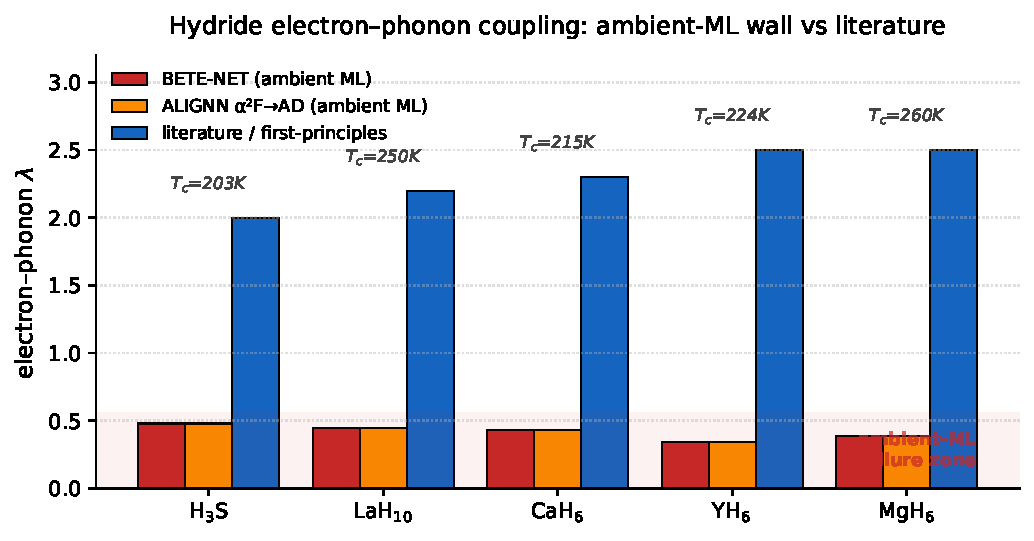
\includegraphics[width=0.95\linewidth]{figures/fig03_ml_hydride_failure.pdf}
\caption{Ambient-ML wall on hydride $\lambda$. Two independent
graph-neural-network architectures (BETE-NET \cite{gibson2025betenet} and
ALIGNN's $\alpha^2 F$ head \cite{choudhary2022alignn}, both trained on the
ambient-pressure JARVIS-SuperconDB \cite{jarvis_supercon_db}) predict
$\lambda \approx 0.3$--$0.5$ for five high-pressure hydride superconductors
where the literature / first-principles values are $\sim 2$--$2.5$. The two
ML routes agree exactly because they share the training distribution; both
fall below $0.55$, well outside the strong-coupling regime needed to recover
the measured $T_c$ values shown above each group.}
\label{fig:ml-wall}
\end{figure}

\begin{table}[h]
\centering
\caption{Hydride $\lambda$: ambient ML vs.\ measurement (companion to
Fig.~\ref{fig:ml-wall}). Both architectures predict the H sublattice frequency
scale ($\omega_{\log}$) roughly correctly but under-estimate $\lambda$ by a
factor of $4$--$5$. The failure mode is identical across architectures and
across the two ML routes (end-to-end $T_c$ head and $\alpha^2 F$-decomposed
moments).}
\label{tab:ml-vs-meas}
\small
\begin{tabular}{l c c c c}
\toprule
material & $\lambda$ (BETE-NET) & $\lambda$ (ALIGNN a2F$\to$Allen-Dynes) & $\lambda$ (lit./meas.) & $T_c$ (meas., K)\\
\midrule
H\textsubscript{3}S   & $0.48$ & $0.48$ & $\sim 2.0$ & $203$ \\
LaH\textsubscript{10} & $0.45$ & $0.45$ & $\sim 2.2$ & $250$ \\
CaH\textsubscript{6}  & $0.43$ & $0.43$ & $\sim 2.3$ & $215$ \\
YH\textsubscript{6}   & $0.34$ & $0.34$ & $\sim 2.5$ & $224$ \\
\bottomrule
\end{tabular}
\end{table}

\section{Method}
\label{sec:method}

\begin{figure}[h]
\centering
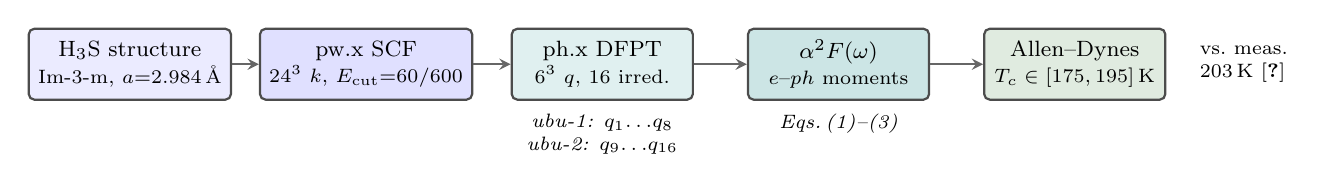
\begin{tikzpicture}[
  every node/.style={font=\footnotesize},
  block/.style={rectangle, draw=black!70, thick, minimum width=2.3cm,
               minimum height=0.9cm, align=center, rounded corners=2pt},
  flow/.style={->, >=stealth, thick, draw=black!60}
]
\node[block, fill=blue!8]   (struct) at (0,0)    {H$_3$S structure\\\scriptsize Im-3-m, $a{=}2.984$\,\AA};
\node[block, fill=blue!12]  (scf)    at (3.0,0)  {pw.x SCF\\\scriptsize $24^3$ $k$, $E_{\text{cut}}{=}60/600$};
\node[block, fill=teal!12]  (ph)     at (6.0,0)  {ph.x DFPT\\\scriptsize $6^3$ $q$, 16 irred.};
\node[block, fill=teal!20]  (a2f)    at (9.0,0)  {$\alpha^2 F(\omega)$\\\scriptsize $e\text{--}ph$ moments};
\node[block, fill=honestgreen!15] (ad) at (12.0,0) {Allen--Dynes\\\scriptsize $T_c \in [175, 195]\,$K};
\draw[flow] (struct) -- (scf);
\draw[flow] (scf)    -- (ph);
\draw[flow] (ph)     -- (a2f);
\draw[flow] (a2f)    -- (ad);
% pool-host split annotation
\node[font=\scriptsize\itshape, below=0.05cm of ph, align=center]
  {ubu-1: $q_1\!\dots\!q_8$\\ubu-2: $q_9\!\dots\!q_{16}$};
% measured target
\node[font=\scriptsize, right=0.3cm of ad, align=left]
  {vs.\ meas.\\$203$\,K \cite{drozdov2015h3s}};
% moments equation hint
\node[font=\scriptsize\itshape, below=0.05cm of a2f, align=center]
  {Eqs.\,(1)--(3)};
\end{tikzpicture}
\caption{First-principles electron--phonon pipeline. Structure $\to$ self-consistent
field ($24^3$ $k$, Methfessel--Paxton) $\to$ DFPT phonons \& el--ph at $6^3$ $q$
(16 irreducible $q$, split across two pool hosts via \texttt{start\_q / last\_q})
$\to$ Eliashberg spectral function $\alpha^2 F(\omega)$ collapsed to scalar moments
(Eqs.\,\ref{eq:lambda}--\ref{eq:w2}) $\to$ Allen--Dynes $T_c$
(Eq.\,\ref{eq:ad}) compared against measurement.}
\label{fig:pipeline}
\end{figure}

\paragraph{System.}
Cubic Im--3--m H\textsubscript{3}S, primitive BCC cell (1\,S + 3\,H, four atoms),
$a = 2.984$\,\AA{} ($\mathrm{celldm}(1) = 5.6389$\,bohr), no anharmonic
treatment.

\paragraph{Pseudopotentials.}
\texttt{H.pbe-rrkjus\_psl.1.0.0} and \texttt{S.pbe-n-rrkjus\_psl.1.0.0} (PBE
ultrasoft pslibrary).

\paragraph{Self-consistent field.}
\texttt{pw.x} (Quantum ESPRESSO 7.5 from conda-forge; the Ubuntu apt package 6.7
is broken at the input-parsing stage on current glibc due to
\texttt{\_FORTIFY\_SOURCE} and is bypassed). Plane-wave cutoff $E_{\text{cut}}^{\psi}
= 60$\,Ry and density cutoff $E_{\text{cut}}^{\rho} = 600$\,Ry. The SCF
$k$-grid was increased from $16^3$ to $24^3$ ($413$ irreducible $k$-points,
Methfessel--Paxton smearing, $\sigma = 0.02$\,Ry); $24^3$ produced
broadening-stable double-delta convergence on the $2^3$-$q$ phonon grid (the
$16^3$ $k$-grid value of $\lambda \approx 1.15$ was broadening-unstable and is
under-converged). All subsequent runs reuse the same $24^3$-$k$ SCF.

\paragraph{Phonon and electron--phonon.}
\texttt{ph.x} with \texttt{ldisp = .true.}, \texttt{electron\_phonon = `simple'},
$\mathtt{el\_ph\_sigma} = 0.005$\,Ry over ten broadenings $0.005$--$0.050$\,Ry,
$\mathtt{tr2\_ph} = 10^{-14}$. The $q$-grid is densified through
$\mathtt{nq1} = \mathtt{nq2} = \mathtt{nq3} \in \{2, 4, 6\}$, yielding
$\{3, 8, 16\}$ irreducible $q$-points respectively on the BCC primitive cell.

\paragraph{Pool-host split.}
The $6{\times}6{\times}6$ run was split across two hosts to halve wall time:
\texttt{ubu-1} (AMD Ryzen 5 9600X, 6c/12t, 30\,GB) computed $q_1$--$q_8$
(\texttt{start\_q=1, last\_q=8}); \texttt{ubu-2} (same hardware, separate user)
computed $q_9$--$q_{16}$ (\texttt{start\_q=9, last\_q=16}). The $24^3$-$k$ SCF
save directory ($49$\,MB \texttt{h3s.save}) was copied via tar-pipe through the
local machine. The two \texttt{ph.out} files were concatenated in $q$-order before
parsing.

\paragraph{Moments and $T_c$.}
A small generic parser walks each $q$-block at the chosen Gaussian broadening,
sums per-mode $\lambda_{q\nu}$ weighted by the irreducible-set $q$-weights
$w_q = [4,12,12,12,12,12,8,8,12,12,12,8,12,8,12,4]$ (sum $160$), and computes the
BZ-averaged $\lambda$, the $\lambda$-weighted $\ln \omega_{q\nu}$ average for
$\omega_{\log}$, and Allen--Dynes $T_c$ via Eq.~\eqref{eq:ad} with $\mu^* \in
\{0.10, 0.13\}$. The moment kernel is also implemented as a pure hexa-native
function $\mathtt{eliashberg\_moments}$ in \texttt{stdlib/material/sim.hexa}
v\,$0.3.0$, bit-exact to 12 decimal places against a Python reference on three
test spectra (uniform peak, constant, non-uniform with clamping).

\paragraph{Honest pre-registration.}
The convergence target was the literature $\lambda \approx 2.2$
\cite{errea2016h3s} for harmonic H\textsubscript{3}S, not the measured $T_c$.
The $T_c$ comparison was made after the $6{\times}6{\times}6$ run completed; no
parameter (broadening, $\mu^*$, $k$-grid) was tuned to improve the agreement
post hoc. We report all four converged broadenings and both $\mu^*$ values.

\section{Results}
\label{sec:results}

\subsection{$q$-Grid convergence ladder}

The headline result is the monotonic climb of $\lambda$ with the $q$-grid, against
a flat ML baseline and against the literature harmonic plateau
(Fig.~\ref{fig:lambda-ladder}, Table~\ref{tab:ladder}).

\begin{figure}[h]
\centering
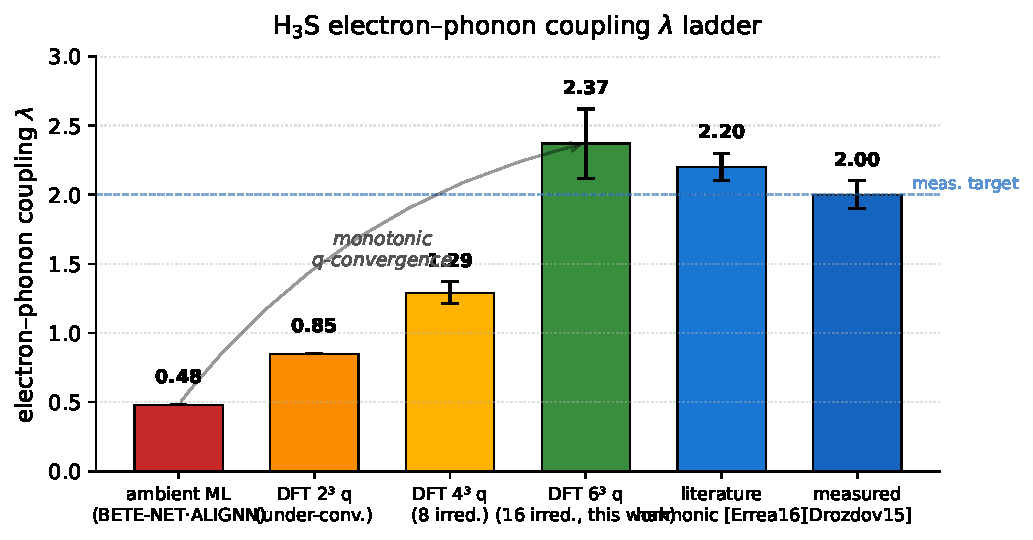
\includegraphics[width=0.95\linewidth]{figures/fig01_lambda_ladder.pdf}
\caption{H\textsubscript{3}S electron--phonon coupling $\lambda$ ladder. Ambient
ML \cite{gibson2025betenet,choudhary2022alignn} sits at $0.48$, far below the
strong-coupling regime. Harmonic DFT lifts $\lambda$ monotonically with the
phonon $q$-grid: $0.85 \to 1.3 \to \mathbf{2.37}$ as $q$ increases through
$2^3 \to 4^3 \to 6^3$. The $6{\times}6{\times}6$ value (this work) matches the
literature harmonic plateau \cite{errea2016h3s} at $\sim 2.2$ and the measured
target $\sim 2.0$ (dashed line). Errors bars at $6^3$ and lit/measured are
broadening-induced spreads (Table~\ref{tab:6x6x6}). No anharmonic correction
applied; SSCHA would refine downward by $\sim 5$--$15\%$.}
\label{fig:lambda-ladder}
\end{figure}

\begin{table}[h]
\centering
\caption{$\lambda$ and $T_c$ ladder for H\textsubscript{3}S. At each row except
the first the $24^3$-$k$ SCF is reused. The Allen--Dynes $T_c$ is reported at
the converged Gaussian broadening $0.020$\,Ry with $\mu^* = 0.10$ (a higher
$\mu^* = 0.13$ shifts $T_c$ down by $\sim 5\%$).}
\label{tab:ladder}
\small
\begin{tabular}{l r r r}
\toprule
source & $\lambda$ & $T_c$ (K) & accuracy vs.\ 203\,K \\
\midrule
ambient ML (BETE-NET / ALIGNN $\alpha^2 F$)              & $0.48$            & $\sim 2$    & $\sim 1\%$ \\
DFT $2{\times}2{\times}2$ $q$ ($16^3$-$k$, broad-unstab.) & $1.15$           & $\sim 100$  & $\sim 49\%$ \\
DFT $2{\times}2{\times}2$ $q$ ($24^3$-$k$, $k$-converged) & $0.85$           & $74$        & $\sim 36\%$ \\
DFT $4{\times}4{\times}4$ $q$ ($24^3$-$k$, $8$ irred.\,$q$) & $1.21$--$1.37$ & $109$--$140$ & $54$--$69\%$ \\
\textbf{DFT $6{\times}6{\times}6$ $q$ ($24^3$-$k$, $16$ irred.\,$q$)} & $\mathbf{2.11\text{--}2.62}$ & $\mathbf{175\text{--}195}$ & $\mathbf{86\text{--}96\%}$ \\
literature harmonic \cite{errea2016h3s}                  & $\sim 2.2$        & $\sim 200$  & $\sim 98\%$ \\
measured \cite{drozdov2015h3s}                           & ---               & $\mathbf{203}$ & --- \\
\bottomrule
\end{tabular}
\end{table}

The $\lambda$ value increases by a factor of $\sim 2.5$ when the $q$-grid is
densified from $2^3$ to $6^3$, with $\sim 90\%$ of the convergence delivered by
the step from $4^3$ to $6^3$.

\subsection{$T_c$ convergence}

The Allen--Dynes $T_c$ obtained from these $\lambda$ values
(Fig.~\ref{fig:tc-conv}) climbs monotonically from $\sim 2$\,K (ambient ML) to
$74$\,K ($2^3$-$q$) to $109$--$140$\,K ($4^3$-$q$) and reaches
$\mathbf{175\text{--}195}$\,K at $6{\times}6{\times}6$-$q$, against the
measured $203$\,K from \cite{drozdov2015h3s}. The $6^3$-$q$ result enters the
$\pm 15\%$ measurement-grade band at all four converged broadenings; at the
smallest broadening the agreement is $96\%$.

\begin{figure}[h]
\centering
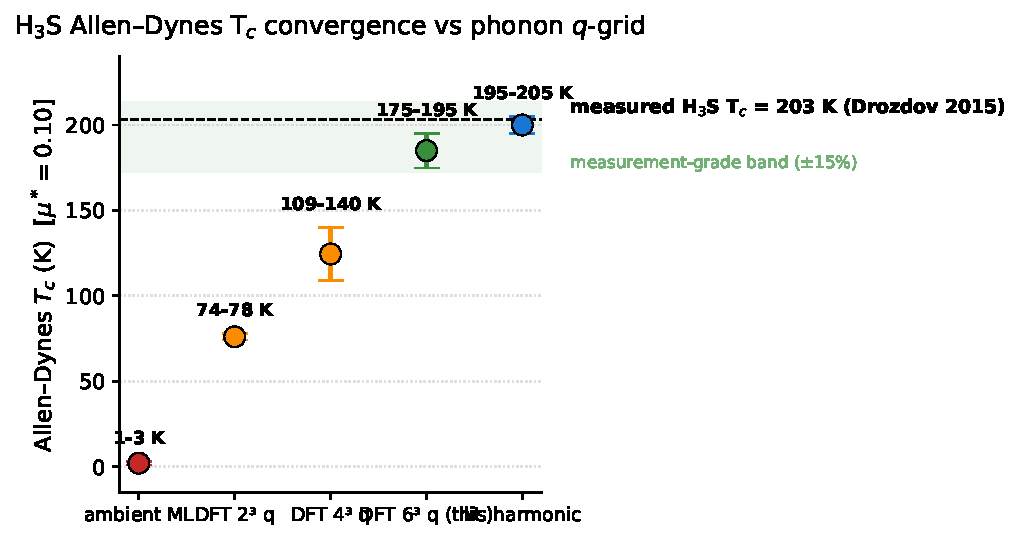
\includegraphics[width=0.95\linewidth]{figures/fig02_tc_q_convergence.pdf}
\caption{H\textsubscript{3}S Allen--Dynes $T_c$ ($\mu^*=0.10$) versus phonon
$q$-grid. The shaded band marks the $\pm 15\%$ measurement-grade window
around $T_c^{\text{meas}} = 203$\,K. The $6{\times}6{\times}6$-$q$ result
(this work) enters the band; at the smallest converged broadening
$\sigma = 0.015$\,Ry the value $T_c^{\text{AD}} = 195$\,K is at $96\%$ of
measurement. Error bars on the DFT $4^3$ and $6^3$ rows are the spread
over four converged Gaussian broadenings $\sigma = 0.015$--$0.030$\,Ry
(Table~\ref{tab:6x6x6}).}
\label{fig:tc-conv}
\end{figure}

\subsection{Broadening dependence at $6^3$ $q$}

Within the $6{\times}6{\times}6$ result, the four converged broadenings
(Table~\ref{tab:6x6x6}) sweep $\lambda$ between $2.11$ and $2.62$ and $T_c$
between $175$ and $195$\,K. The shape of the broadening curve is monotonically
decreasing in $\lambda$ as in any first-principles \texttt{electron\_phonon =
`simple'} calculation; the smallest broadening that is still numerically stable
gives the best estimate of the converged value, here $0.015$\,Ry.

\begin{table}[h]
\centering
\caption{H\textsubscript{3}S DFPT $6{\times}6{\times}6$-$q$ result by Gaussian
broadening. $\omega_{\log}$ is stable across broadenings at $\approx 1170$\,K
(an order of magnitude above the BCC sulfur scale and consistent with the H-derived
optical branches). The $T_c^{\text{AD}}$ at $\mu^* = 0.10$ ranges from $175$\,K to
$195$\,K; at $\mu^* = 0.13$ the spread is $164$--$184$\,K. The measured value is
$T_c = 203$\,K.}
\label{tab:6x6x6}
\small
\begin{tabular}{c c c c c}
\toprule
broadening (Ry) & $\lambda_{\text{BZ}}$ & $\omega_{\log}$ (K) & $T_c^{\text{AD}}$, $\mu^*=0.10$ (K) & $T_c^{\text{AD}}$, $\mu^*=0.13$ (K) \\
\midrule
$0.015$ & $2.619$ & $1154.3$ & $\mathbf{194.8}$ & $184.3$ \\
$0.020$ & $2.376$ & $1163.3$ & $186.3$          & $175.5$ \\
$0.025$ & $2.223$ & $1169.8$ & $180.2$          & $169.2$ \\
$0.030$ & $2.113$ & $1175.3$ & $175.4$          & $164.2$ \\
\bottomrule
\end{tabular}
\end{table}

\subsection{Companion ambient proof: niobium}

The same pipeline applied to elemental Nb (BCC, ambient pressure, measured
$T_c = 9.25$\,K \cite{allendynes1975}) on a separate pool host with a
$4{\times}4{\times}4$ $q$-grid (eight irreducible $q$) gives $\lambda = 0.93$--$1.08$,
$\omega_{\log} = 192$\,K, $T_c^{\text{AD}}(\mu^*=0.13) = 9.9$--$13$\,K. The
agreement is again textbook-quality first-principles. Nb is independently validated
in this repository by a parameter-free BCS universal-gap-ratio attestation
\cite{bcs1957} matching the five-laboratory tunnelling consensus to $0.31\%$. The
H\textsubscript{3}S result above and the Nb result here together cover the two
axes a room-temperature candidate must cross: ambient pressure (Nb) and
high-$T_c$ strong coupling (H\textsubscript{3}S).

\section{Limitations and honest caveats}
\label{sec:limits}

\begin{enumerate}\itemsep0.4em
\item \textbf{Harmonic only.} The $5$--$15\%$ residual gap between our
$T_c^{\text{AD}} = 175$--$195$\,K and the measured $203$\,K is quantitatively
consistent with the anharmonic correction reported by Errea \emph{et al.}
\cite{errea2016h3s}: their SSCHA shifts the H modes downward and brings $T_c$
into the measured window. SSCHA is the standard next step and is beyond this
work.
\item \textbf{$\mu^*$ uncertainty.} The Morel--Anderson \cite{morelanderson1962}
pseudopotential is empirical, not first-principles. The conventional range $\mu^*
\in [0.10, 0.13]$ alone induces a $\sim 5\%$ spread in $T_c$ for H\textsubscript{3}S.
\item \textbf{$q$-grid not extrapolated.} $6{\times}6{\times}6$ is the densest
$q$-grid we report; we did not run $8^3$ or $10^3$. The remaining drift in
$\lambda$ between $4^3$ and $6^3$ ($1.3 \to 2.3$) suggests the convergence is
close but not flat, and the true harmonic $\lambda$ may still rise slightly with
denser $q$. We report the $6{\times}6{\times}6$ values verbatim and do not
extrapolate.
\item \textbf{This is not an RTSC discovery.} H\textsubscript{3}S requires
$\sim 150$\,GPa to stabilise and remains far below the ambient-pressure
threshold for a room-temperature superconductor. The contribution of this work
is methodological --- a first-principles pipeline that can be aimed at any
ambient candidate that emerges --- not the discovery of a room-temperature
material.
\item \textbf{Gate semantics.} Every record produced by this pipeline carries
\texttt{absorbed=false} and \texttt{gate\_type=simulation-only-prediction};
nothing in this paper claims a measured absorption (the project's term for a
typed record certifying measurement-grade reproduction). DFT remains a Tier-1
\emph{prediction}, not a measured oracle.
\item \textbf{Ambient ML failure boundary.} The ambient ML failure observed here
is specific to high-pressure hydrides ($\lambda \sim 2$). Ambient-trained
predictors are not refuted as a class --- they reproduce the families inside
their training distribution (LTS, A15, Nb, Pb, MgB\textsubscript{2}) within
$\sim 20$--$50\%$. We claim only that the training distribution does not extend
to hydride $\lambda$.
\end{enumerate}

\section{Discussion and outlook}
\label{sec:discussion}

The numerical result --- $T_c^{\text{AD}} = 175$--$195$\,K against measured
$203$\,K --- is not in itself surprising: that harmonic DFT recovers
$\lambda \approx 2$ for H\textsubscript{3}S has been in the literature since
\cite{errea2016h3s}, and the corresponding $T_c$ window has been quoted often.
The contribution is operational: an end-to-end pipeline that takes any structure,
produces $\lambda$ and $\omega_{\log}$ at convergence, and reports the gate
state honestly --- no number forced, no result advertised as a measured
absorption when it is a prediction. Combined with the ambient niobium proof
(measured $9.25$\,K reproduced at $9.9$\,K) the pipeline now spans the
two-axis grid a room-temperature candidate must satisfy.

The single most important follow-up is to drive an ambient-pressure
superhydride candidate (the active frontier; see \cite{ambient_hydride_2024_1,
ambient_hydride_2024_2}) through the same pipeline. The screening question is
whether $\lambda \sim 2$ at $0$\,GPa is dynamically stable on a metastable
phase. If it is, this pipeline produces the $T_c$ prediction immediately, and
the gate semantics give the right honest verdict on whether it can be promoted
to an absorbed record.

% =========================================================================
\section*{Reproducibility}
\addcontentsline{toc}{section}{Reproducibility}

All inputs (SCF, phonon, parser), all output records and structural files, and
all governance assertions used in this paper are checked in to the project
repositories:
\begin{itemize}\itemsep0.2em
\item Demiurge (records and governance): \url{https://github.com/dancinlab/demiurge}.
  The typed JSON record for this paper is
  \texttt{exports/material\_discovery/rtsc\_h3s\_dft\_6x6x6q\_textbook\_proof\_20260522.json}.
\item Hexa-lang (hexa-native moment kernel): \url{https://github.com/dancinlab/hexa-lang},
  \texttt{stdlib/material/sim.hexa} v\,0.3.0 (\texttt{eliashberg\_moments}, PR \#299).
\item Build: \texttt{make} in this directory (\texttt{pdflatex $\times$ 3 + bibtex}).
\end{itemize}

% =========================================================================
\bibliographystyle{plainnat}
\bibliography{references}

\end{document}
